\section{Video Prediction for Control}
\label{sec:model}

\begin{figure}[t]
	\centering
	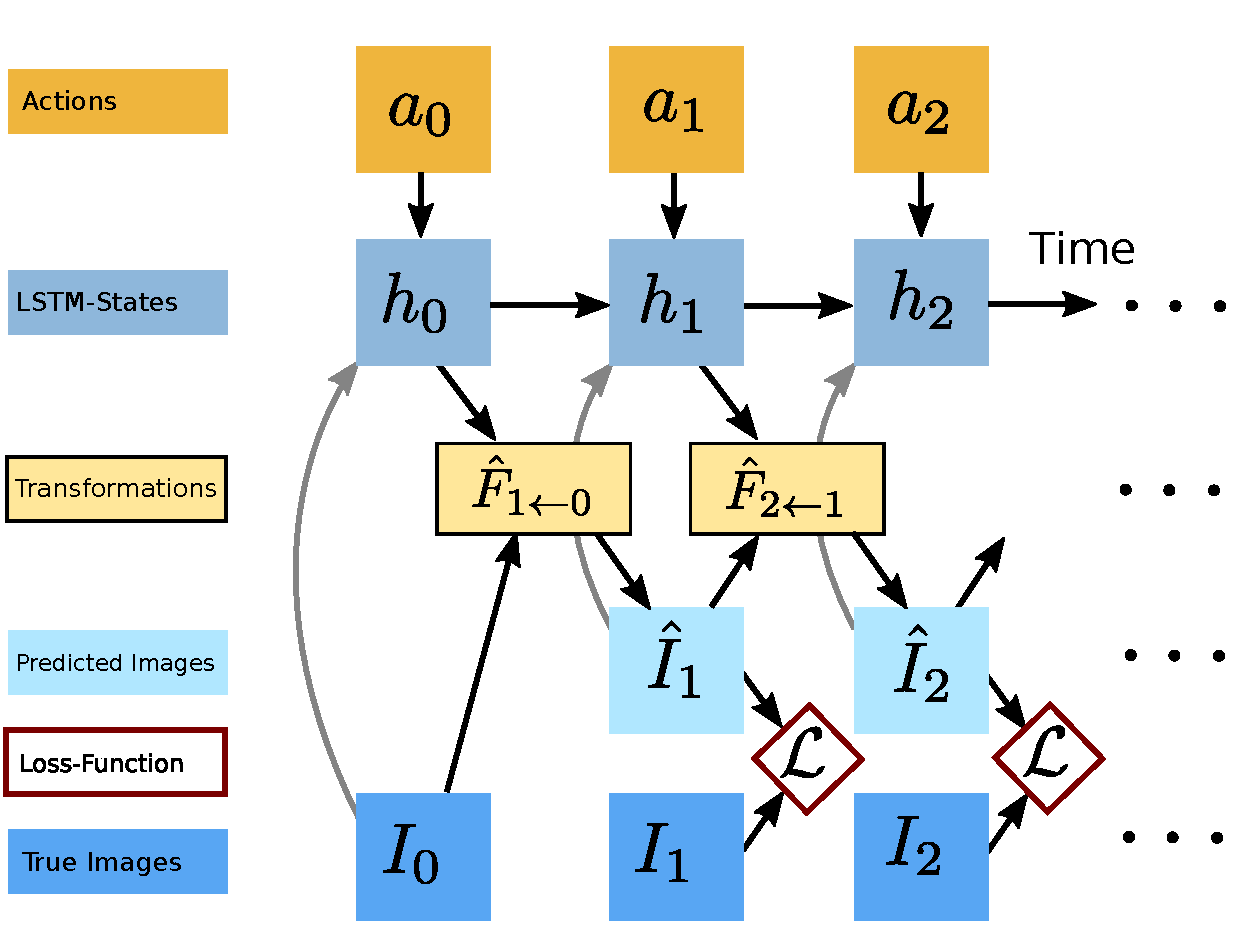
\includegraphics[width=0.7\columnwidth]{images_general/prediction_model.pdf}
	\caption{\small{Computation graph of the video-prediction model. Time goes from left to right, $a_t$ are the actions, $h_t$ are the hidden states in the recurrent neural network, $\hat{F}_{t+1 \leftarrow t}$ is a 2D-warping field, $I_t$ are real images, and $\hat{I}_t$ are predicted images, $\mathcal{L}$ is a pairwise training-loss.}}   
	\label{fig:prediction_model}
\end{figure}

In visual-MPC we use a transformation-based video-prediction architecture, first presented in \cite{finn_nips}. The advantage of using transformation based-models over a model that directly generates pixels, is that prediction is easier when only few objects in the image move by relatively small amounts and also the transformations can be leveraged to obtain predictions of \emph{where} certain pixels in the image are moving, a property that is used in several of our planning cost-function formulations. The model, which is implemented as a recurrent neural network $g_{\theta}$ parameterized by $\theta$, has a hidden state $h_t$ and takes in a previous image and an action at each step of the rollout. Future images $\hat{I}_{t+1}$ are generated by warping the previous generated image $\hat{I}_t$ or the previous true image $I_t$, when available, according to a 2-dimensional flow field $\hat{F}_{t+1 \leftarrow t}$. A simplifying illustration of model's structure is given in figure \ref{fig:prediction_model}. It is also summarized in the following two equations:

\begin{align}
[h_{t+1}, \hat{F}_{t+1 \leftarrow t}] 	&= g_{\theta}(a_t, h_t, I_t) \\
\hat{I}_{t+1} 							&= \hat{F}_{t+1 \leftarrow t} \diamond  \hat{I}_t 
\label{simple_dna}
\end{align}

Here bilinear sampling operator $\diamond$ interpolates the pixel values bilinearly with respect to a location $(x,y)$ and its four neighbouring pixels in the image, similar to \cite{zhou2016view}. Note that as shown in figure \ref{fig:prediction_model}, at the first time-step the real image is transformed, whereas at later timesteps previously generated images are transformed. The model is trained by standard backpropagtion-through time by performing gradient descent on a mean-squared error type image reconstruction loss, denoted by $\mathcal{L}$ in figure \ref{fig:prediction_model}.
\begin{figure}[t]
    \centering
    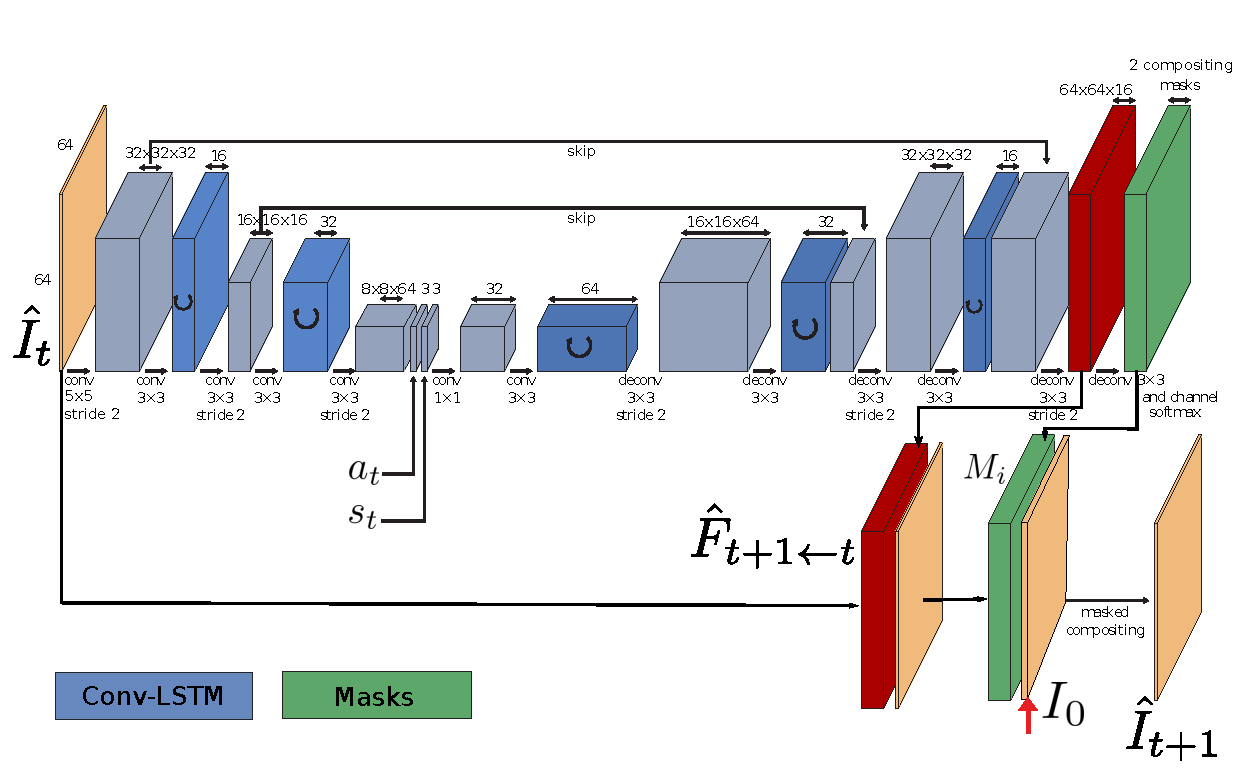
\includegraphics[width=\columnwidth]{images_sna/occlusionaware/architecture.pdf}
    \caption{\small{Forward pass through the recurrent SNA model based on \autoref{eqn:simplemodel}. The red arrow indicates where the image from the first time step $I_0$ is concatenated with the transformed images $\hat{F}_{t+1 \leftarrow t} \diamond  \hat{I}_t $ multiplying each channel with a separate mask to produce the predicted frame for step $t+1$.}}      \label{fig:occlusion_model}
\end{figure}

\label{subsec:pixel_trafo}
A forward pass of the RNN is illustrated in figure \ref{fig:occlusion_model}. We use a series stacked convolutional LSTMs and standard convolutional layers interleaved with average-pooling layers. The result of this computation is the 2 dimensional flow-field $\hat{F}_{t+1 \leftarrow t}$ which is used to transform a current image $I_t$ or $\hat{I}_t$.

\textbf{Predicting motion of individual pixels}: 
When using visual-MPC with a cost-function based on start- and goal pixel positions, a model is required that can effectively predict the 2-D motion of the user-selected start pixels $\pixel_0^{(1)}, \dots, \pixel_0^{(P)}$ up to $T$ steps into the future. Since the model we employ is transformation based, this motion prediction capability emerges implicitly, and therefore no external pixel motion supervision is required. To predict the future positions of the designated pixel $d$, the same transformations which are used to transform the images are applied to the distribution over designated pixel locations. The warping transformation $\hat{F}_{t+1 \leftarrow t}$ can be interpreted as a stochastic transition operator allowing us to make probabilistic predictions about future locations of individual pixels:

\begin{equation}
\hat{P}_{t+1} = \hat{F}_{t+1 \leftarrow t} \diamond  \hat{P}_t
\label{eqn:prob_forward}
\end{equation}

Here $P_t$ is a distribution over image locations which has the same spatial dimension as the image. For simplicity we assume that we only use a single designated pixel. At the first time step the distribution $\hat{P}_0$ is defined as 1 at the position of the user-selected designated pixel and zero elsewhere. The distribution $\hat{P}_{t+1}$ is normalized at each prediction step.

Since this basic model, which we refer to as dynamic neural advection (DNA) model, predicts images only based on the previous image, it is unable to recover shapes (e.g., objects) after they have been occluded, for example by the robot arm. Therefore, this model is only suitable for planning motions where the user-selected pixels are not occluded during the manipulation, which restricts its use in cluttered environments or with multiple selected pixels. In the next section, we introduce an enhanced type of model, which lifts this limitation by employing temporal skip connections.

Note that when using a planning cost function that does not depend on the prediction of pixel positions, like a classifier-based cost function, as detailed in section \ref{subsec:class_cost}, we do not require the model to output transformations and virtually any video prediction model can be used. 

\textbf{Skip Connection Neural Advection Model}
To enable effective tracking of objects through occlusions, we can extend the model discussed in the previous section with temporal skip connections: we now transform pixels not only from the previously generated image $\hat{I}_t$, but from all but from all previous images $\hat{I}_1,...\hat{I}_{t}$, including the context image $I_0$, which is a real image. All these transformed images can combined to a form the predicted image $\hat{I}_{t+1}$ by taking a weighted some over all transformed images, where the weights are given by masks $\mathbf{M}_t$ with the same size as the image and a single channel:
\begin{equation}
\hat{I}_{t+1} =  \mathbf{M}_{0} (\hat{F}_{t+1 \leftarrow 0} \diamond I_t) +  \sum_{j=1}^{\tau} \mathbf{M}_{j} (\hat{F}_{t+1 \leftarrow j} \diamond  \hat{I}_j).
\end{equation}

We refer to this model as the \emph{skip connection neural advection model (SNA)}, since it handles occlusions by using temporal skip-connections such that when a pixel is occluded (e.g., by the robot arm or by another object) it can still reappear later in the sequence.

Transforming from all previous images comes with increased computational cost, since the number of masks and transformations scales with the number of time-steps $\tau$. However, we found that in practice a greatly simplified version of this model, where transformations are applied only to the previous image and the \emph{first image} of the sequence $I_0$ works equally well. Moreover we found that transforming the first image of the sequence is not necessary, as the model uses its pixels primarily to generate the image background. Therefore, we can use the first image directly, without transformation, such that
\begin{equation}
\hat{I}_{t+1} = \mathbf{M}_{0} I_0 +  \mathbf{M}_{1} (\hat{F}_{t+1 \leftarrow t} \diamond \hat{I}_t).
\label{eqn:simplemodel}
\end{equation}
Here, we make the assumption that occluded objects are static throughout the prediction horizon. This assumption allows us to dispense the intermediate transformations and only provide a skip connection from the very first image in the sequence $I_0$, which is also the only real image, since all of the subsequent images are predicted by the model. Hence, this model only needs to output 2 masks. 


%\todo{can cut from here:}
%Next, we show another illustration comparing the occlusion handling of DNA and the proposed SNA model. The graphs in \autoref{fig:pix_reqppear_graph} show the predicted probability evaluated at the position of the designated pixel, shown in figure \ref{fig:desig_pix_bluedot}, which is stationary during the entire motion. Precisely when the arm occludes the designated pixel, the probability at this point decreases. This indicates that the model is `unsure' where this pixel is. When the arm unoccludes the designated pixel, it should become visible again, and the probability of the designated pixel being at its original position should go up. In the case of the DNA model and its variants~\cite{finn_nips}, the probability mass does not increase after the object reappears. 
% 
% \begin{figure}[t]
% 	\centering
% 	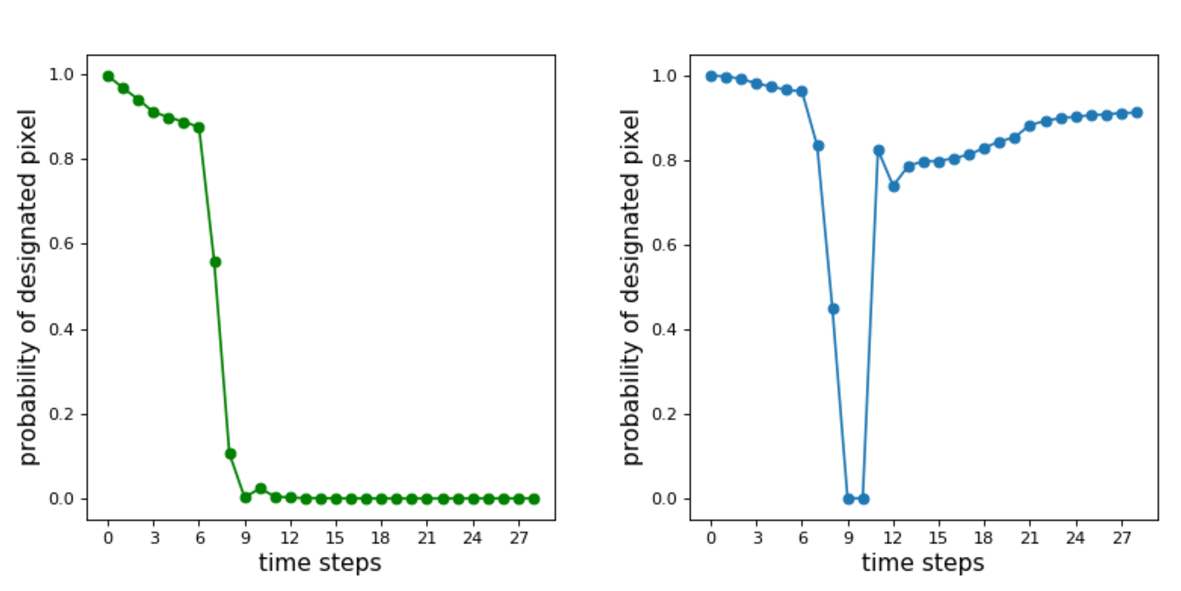
\includegraphics[width=0.9\columnwidth]{images_sna/occlusionaware/probability_curves.pdf}
% 	\caption{Predicted probability $P_{d^{(0)}}(t)$ of the designated pixel being at the location of the blue dot indicated in \autoref{fig:desig_pix_bluedot} for the DNA model (left) and the SNA model (right). \todo{can cut if no more space!}}      \label{fig:pix_reqppear_graph}
% \end{figure}

